\begin{figure}
  \centering
  % \resizebox{\columnwidth}{!}{
  %   \begin{tikzpicture}
  %
  % Define basic styles
  %
  % Node
  \tikzstyle{module} = [draw, very thick, rounded corners,
  fill=white, minimum height=2.5em, inner sep=0.5em,
  rectangle, font={\bfseries}, align=center]
  \tikzstyle{cmodule} = [module, fill=black!20]

  % Edge
  \tikzstyle{stateEdgePortion} = [black, thick];
  \tikzstyle{dataEdge} = [stateEdgePortion, ->];
  \tikzstyle{controlEdgePartial} = [stateEdgePortion, dashed];
  \tikzstyle{controlEdge} = [controlEdgePartial, ->];
  \tikzstyle{controlDoubleEdge} = [controlEdgePartial, <->];
  \tikzstyle{edgeLabel} = [pos=0.5, text centered, font={\itshape}];

  \node[name=client, draw, very thick, fill=white,
  double copy shadow={shadow xshift=2pt, shadow yshift=-2pt, fill=white, draw},
  text height=13em, text width=31.5em] {};

  \node[name=server, draw, very thick, fill=white, draw,
  right=of client.north east, anchor=north west, xshift=1em,
  text height=7em, text width=12.5em] {};

  \node[module, name=source, below right=of client.north west,
  xshift=-1.5em, yshift=1.5em] {Source};
  \node[module, name=transform, right of=source, xshift=3.5em] {Transform};
  \node[cmodule, name=degrade, right of=transform, xshift=3.7em] {Degrade};
  \node[cmodule, name=queue, right of=degrade, xshift=3em] {Queue};
  \node[cmodule, name=socket, right of=queue, xshift=3em, text width=3em] {Socket};
  \node[cmodule, name=receiver, right of=socket, xshift=7em] {Receiver};
  \node[module, name=analytics, right of=receiver, xshift=3em] {Analytics};

  \node[cmodule, name=cc, at=($(queue)!0.5!(socket)$), yshift=-6em]
  {Congestion\\Controller};

  \draw ($(source.east)$) edge[dataEdge] ($(transform.west)$);
  \draw ($(transform.east)$) edge[dataEdge] ($(degrade.west)$);
  \draw ($(degrade.east)$) edge[dataEdge] ($(queue.west)$);
  \draw ($(queue.east)$) edge[dataEdge] ($(socket.west)$);
  \draw ($(socket.east)$) edge[dataEdge] node[edgeLabel, yshift=0.6em] {data}
  ($(receiver.west)$);
  \draw ($(receiver.east)$) edge[dataEdge] ($(analytics.west)$);

  %% Control path
  \draw let
  \p1 = ($(cc.center)$), \p2 = ($(degrade.center)$)
  in ($(cc.west)$) edge[controlEdgePartial] (\x2, \y1)
  (\x2, \y1) edge[controlEdge] ($(degrade.south)$);

  \draw let
  \p1 = ($(queue.south)$), \p2 = ($(cc.north)$)
  in ($(\x1, \y1) + (1em,0)$) edge[controlEdge] ($(\x1, \y2) + (1em,0)$);

  \draw let
  \p1 = ($(socket.south)$), \p2 = ($(cc.north)$)
  in ($(\x1, \y1) + (-1em,0)$) edge[controlDoubleEdge] ($(\x1, \y2) + (-1em,0)$);

  \node[name=clientlabel, above right=of client.south west, xshift=-2em, yshift=-2em] {Edge (Client)};
  \node[name=clientlabel, above left=of server.south east, xshift=2em, yshift=-2em] {Server};

  %%
  %% Legend
  %%
  \node[name=datalegend, below=1.5em of server.south west, xshift=2em]
  {\small Data Plane};
  \draw ($(datalegend.west) + (-2em, 0)$) edge[dataEdge]
  ($(datalegend.west) + (-0.5em, 0)$);

  \node[name=controllegend, below=2.5em of datalegend.west, anchor=west]
  {\small Control Plane};
  \draw ($(controllegend.west) + (-2em, 0)$) edge[controlEdge]
  ($(controllegend.west) + (-0.5em, 0)$);

  \node[name=applegend, right=3em of datalegend.east]
  {\small Application Logic};
  \node[module, name=applegendbox, left=0.1em of applegend, text width=0.3em,
  minimum height=0em] {};

  \node[name=syslegend, below=2.5em of applegend.west, anchor=west]
  {\small Runtime};
  \node[cmodule, name=syslegendbox, left=0.1em of syslegend, text width=0.3em,
  minimum size=0em] {};

\end{tikzpicture}

%%% Local Variables:
%%% mode: latex
%%% TeX-master: "sosp17"
%%% End:

  % }
  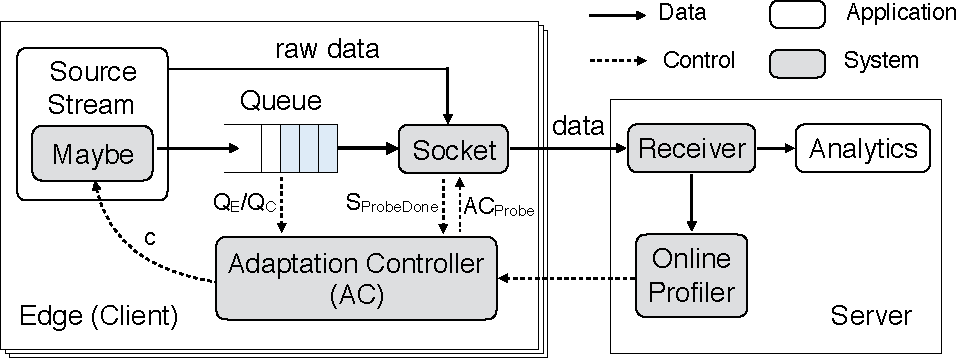
\includegraphics[width=\linewidth]{figures/runtime-adaptation.pdf}
  \caption{Runtime adaptation system architecture.}
  \label{fig:runtime}
\end{figure}

\subsection{Runtime Adaptation}
\label{sec:runtime}

At runtime, \sysname{} performs application adaptation according to the learned
profile. We choose design our own runtime system and adaptation algorithm
because there is no viable system. Network protocols adapts to available
resources without application accuracy guarantee. Video streaming's adaptation
relies on the playback buffer~\cite{huang2014buffer}, incurring high
latency. JetStream~\cite{rabkin2014aggregation} doesn't know the bandwidth
demand of each rule in a policy. It adapts gradually and the slow reaction adds
additional latency.

Our runtime system architecture is shown in \autoref{fig:runtime}. \sysname{}
applications' source contains a \texttt{Maybe} module derived from all \maybe{}
operations. This module allows controller to \textit{update} the level of
degradation. Data generated by the source is then enqueued to \texttt{Queue} and
subsequently dequeued by \texttt{Socket}. When data generation rate exceeds
\texttt{Socket}'s departure rate, the queue grows. At this time, the adaptation
controller (AC) queries the estimated bandwidth from \texttt{Socket} and
regulates the source stream by updating the configuration.  After the data is
sent through the network, the receiver extracts raw data to the online profiler
and delivers data to the application analytics. The raw data is only transmitted
when the queue is empty. When a new profile is learned, it's fed back to AC for
subsequent adaptation.

We then focus on the adaptation algorithm (\autoref{fig:cc}). AC loads the
profile and sorts all configurations with an ascending order of bandwidth
demand, denoted as $[c_1, \dots, c_{max}]$. The current configuration is $c$ and
the next $c_{i+1}$. AC receives message from the \texttt{Queue}: \qe{} for when
the queue is empty and $\text{Q}_\text{C}$ when queued items exceeds a
threshold. AC can query \texttt{Socket} for delivery rate $R$ or request it to
probe for a target bandwidth, often $B(c_{i+1})$. When $R > B(C_{i+1})$,
\texttt{Socket} sends back \spd{}. The algorithm follows a state machine:

\para{Startup: rapid growth.} \sysname{} starts up with $c_1$ and grows the rate
upon each \qe{}. The growth stops at $c_{max}$ (to \texttt{Steady}) or or it
receives \qc{} (to \texttt{Degrade}).

\para{Degrade: reacting to congestion.} When objects are queued, AC receives
\qc{} and runs \texttt{adapt()}. It involves two steps: (1) AC queries $R$ from
\texttt{Socket}; (2) AC updates \texttt{Maybe} with $c$ such that
$B(c) < \alpha R, \alpha \in (0, 1)$. A smaller $\alpha$ allows a quicker
draining of the queue. \sysname{} changes to \texttt{Steady} after the queue is
drained.

\para{Steady: low latency delivery.} \sysname{} achieves low latency by spending
most of the time in \texttt{Steady} state. It changes to \texttt{Degrade} when
congestion occurs. If $c < c_{max}$ and it receives \qe{}, AC enters
\texttt{Probe} state to check for more available bandwidth.

\para{Probe: more bandwidth for a higher accuracy.} Advancing $c$ directly
causes drastic latency increase when $B(c_{i+1}) \gg B(c_i)$. To allow a smooth
increase, AC requests \texttt{Socket} to probe by sending additional traffic
controlled by \texttt{probe\_gain} (in \texttt{inc\_pace()}, similar to
BBR~\cite{cardwell2017bbr}). \sysname{} stops probing under two conditions: (1)
upon \spd{}, it advances the configuration; (2) upon \qc{}, it returns to
\texttt{Steady}.

\begin{figure}
  \begin{subfigure}[t]{\columnwidth}
    \centering
    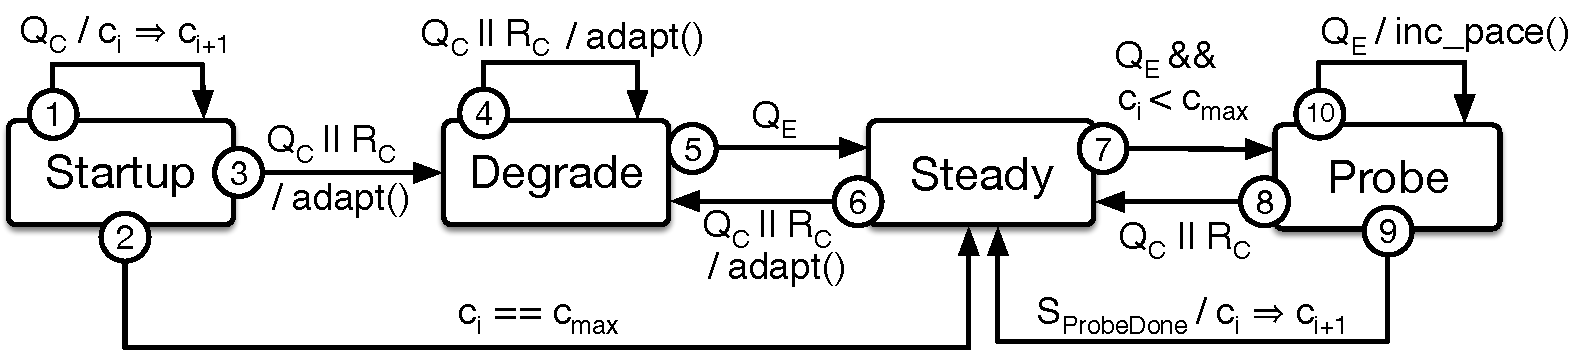
\includegraphics[width=\columnwidth]{figures/cc.pdf}
    \caption{Rate Adaptation State Machine}
    \vspace{1em}
    \label{fig:cc-sm}
  \end{subfigure}
  \begin{subfigure}[t]{0.95\columnwidth}
    \centering
    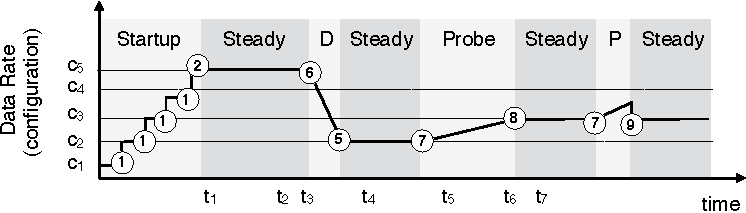
\includegraphics[width=\columnwidth]{figures/cc2.pdf}
    \caption{An example to illustrate the adaptation algorithm.}
    \label{fig:cc-ex}
  \end{subfigure}

  \caption{The adaptation algorithm as a state machine and an illustration of
    one possible trace showing state transitions.}
  \label{fig:cc}
\end{figure}

% \begin{figure}
%   \centering
%   \resizebox{\columnwidth}{!}{
%     \begin{tikzpicture}[
  state/.style = { draw, very thick, fill=white, rounded corners=1em,
    minimum height=3em, minimum width=7em, node distance=7em, font={\bfseries},
    align=center },
  edge portion/.style = { black, thick },
  transition/.style = { edge portion, -> },
  algorithm/.style = { draw, thin, fill=white },
  ]

  \node [state] (startup) {
    STARTUP };
  \node [state] (congestion) [right=of startup] {CONGESTION};
  \draw [transition] (startup) -- (congestion)
  node [midway, auto] {Q.Congestion};

  \node [state] (steady) [below=of congestion] {STEADY};

  \draw [transition] ($(congestion.south west)!0.4!(congestion.south east)$)
  to node[midway, sloped, below] {Q.NoQueue}
  ($(steady.north west)!0.4!(steady.north east)$);

  \draw [transition] ($(steady.north west)!0.6!(steady.north east)$)
  to node[midway, sloped, below] {Q.Congestion}
  ($(congestion.south west)!0.6!(congestion.south east)$);

  \node [state] (probe) [left=of steady] {PROBE};

  \draw [transition] ($(steady.south west)!0.6!(steady.north west)$)
  -- ($(probe.south east)!0.6!(probe.north east)$)
  node[midway, auto, swap] {Q.Probe};

  \draw [transition, <-] ($(steady.south west)!0.4!(steady.north west)$)
  -- ($(probe.south east)!0.4!(probe.north east)$)
  node[midway, auto, align=left] {Q.Congestion | \\ IO.ProbeDone};

\end{tikzpicture}


%%% Local Variables:
%%% mode: latex
%%% TeX-master: "sosp17"
%%% End:

%   }
%   \caption{Congestion Control Algorithm}
%   \label{fig:cc}
% \end{figure}

\vspace{1em}
\noindent\textbf{Resource Allocation and Fairness}

In addition to rate adaptation, the profile is also useful for controlling
bandwidth usages of a single application and allocating resources among
competing tasks.

For individual applications, developers can pinpoint a configuration for a given
bandwidth or accuracy goal. They can also specify criterion to limit effective
configurations. For example, \sysname{} can enforce an upper bound on the
bandwidth consumption. Such a limit is extremely useful when bandwidth usages
incur high cost.

For multiple applications, their profiles allows novel bandwidth allocation
schemes such as utility fairness. Different from traditional resource fairness
where applications get equal share of bandwidth, \textit{utility fairness} aims
to maximize the \textit{minimal} application accuracy. With the profiles,
finding allocations is equivalent of finding proper configuration $c_i^t$ for
application $t$. We formulate utility fairness as follows:

\begin{equation}
  \label{eq:multitask}
    \underset{c_i^t}{\max} \; \min({A^t(c_i^t)})
    \;
    \text{s.t.}
    \;
    \sum_t{B^t(c_i^t)} < R
\end{equation}

Solving this optimization is computationally hard. \sysname{} uses a heuristics
approach. We start with $c_1^t$ and improve the application $t$ that has the
worst accuracy. This process is repeated until all available bandwidth is
allocated.

%%% Local Variables:
%%% mode: latex
%%% TeX-master: "sosp17"
%%% End:
